\section{Methodology}
\label{sec:methods}

\paragraph{Classes of 3D understanding tasks. }
\label{methods:tasks}
We consider three distinct classes of challenging part-level 3D scene understanding tasks: semantic labeling, hierarchical semantic segmentation, and instance segmentation. 
The input to all our models is the voxelized scene SDF, representing 3D geometry without associated RGB values.

In~\emph{semantic labeling,} the goal is to associate a set of $n$ semantic part labels~$y_j = (y_j^{d_1}, \ldots, y_j^{d_n})$ with each voxel~$v_j$, 
at detail levels~$d_1, \ldots, d_n$.
To predict parts in such multi-label formulation, we produce a set of softmax scores $p_j = (p_j^{d_1}, \ldots, p_j^{d_n})$.
We train the network in multiple setups, differing by the structure of supervision available to the network, each time evaluating labeling performance at each detail level $d_i$. Specifically, we define 
our loss function $L$ to be a weighted sum of cross entropy losses for each level of detail
\begin{equation}
\label{eq:semseg_loss}
L(p, y) = \sum_{k = 1}^K \alpha_k L_{\text{CE}}(p^k, y^k)
\end{equation}
and specify a set of weighting schemes for $\alpha_1, \ldots, \alpha_K$. 
This loss structure allows expressing both ``flat'' segmentation formulations (e.g., choosing $\alpha_{k} = \delta_{ki}$ to segment at level $d_i$ only), that we view as baselines, and multi-task formulations that integrate training signal across multiple levels of semantic detail.

For this task we 

To perform \emph{hierarchical semantic segmentation,} one must perform segmentation at multiple levels in the hierarchy, inferring labels in coarse- and fine-grained detail levels simultaneously. 
Similarily to~\cite{mo2019partnet}, we approach this task using \emph{bottom-up,} \emph{top-down} and \emph{ensemble} method.
Bottom-up method performs segmentation at the most fine-grained level and propagates the labels to object level, leveraging the taxonomy structure.
Conversely, the top-down approach infers labels first at coarse level (starting with objects) and subsequently at finer levels (parts), recursively descending along predicted taxonomy branches.
With the ensemble method, predictions of networks independently trained at distinct detail levels are integrated in a joint inference step.
We note that \emph{multi-task training} using~\eqref{eq:semseg_loss} also results in a hierarchical segmentation method, and include it in the comparison.






% we use a set of linear layers and project voxel features to labels, producing

% The model assigns the input  to several classes \DZ{unclear -- one of several classes?  what is depending on what?}  depending on the total number of part classes on the selected level of detail (LoD) of objects part taxonomy.
% The distribution of class labels on all of LoDs is very unbalanced, as shown on the treemap diagram \ref{fig:class_distribution_treemap}.
% On a given level of detail $k$, the frequency of  a voxel class $i=0 \ldots N^k$ is denoted $C_i^k$.  Then the Cross Entropy loss function weights for class $i$ are equal to $w_i^k = \frac{\max_{i=0 \ldots N^k} (C_i)}{C_i}$.
% If the model is trained to predict labels for several levels of detail $\{k,n,p\}$ we use multiple linear layers to project each voxel features to labels. The final loss function $L$ is computed as a weighted sum of Cross Entropy losses for each level of detail: 
% \[L = \sum_{j\in\{k,n,p\}} w_j L_j
% \]

% flat softmax at lod=1,2,3, and multiloss(12, 123), with quality computed separately (+bottom up deduced labels), +topdown with own softmax labels with masking all of the other labels: here inference would be, choose heads which are predicted as positive, and go one level down inferring, ensemble 


% — В этой работе в качестве отправной точки мы выбрали реализацию двух подходов, topdown и bottomup, в качестве двух основных стратегий интеграции разметки на различных уровнях детализации. 
% — Кроме того, мы исследуем различные схемы взвешивания сигналов на разных уровнях таксономии, неявно кодирующие редукцию таксономии.

% Overall, semantic and hierarchical segmentation tasks have been considered in multiple settings:
% \begin{enumerate}
% \item Bottom-up approach: Segmentation of part labels on different levels of detalization from object level to 3 levels of hierarchy down
% %\textcolor{blue}{VI: Первое упонимание о трех уровнях иерархии частей, хотя на данном этапе нет ни одного упонимания датасета. Вероятно, лучше описание датасета поместить перед методологией (в Scan2CAD сначала идёт описание датасета).}
% , which, in turn, allows us to compute predictions for higher labels.% this approach sometimes called "Bottom-Up".

% \item Top-down approach:  each sub-part segmentation is performed in parallel in separate linear projections from voxel features (masked by ground truth of parent part labels).
% \DZ{why is this top-down?} \AN{In test-time predictions computed from root node of hierarchy and then depending on the predicted classes sub-part classified by the "head" dedicated to that node, it does that until terminal node (leaf) is reached.} \DZ{Ok I got the explanation above, but still do not understand the linear projection part; I leave it to AN or AA to rewrite}

% \item Ensemble Segmentation \cite{mo2019partnet}  on all levels at the same time, projecting the voxel features to 3 different heads and testing different weighting schemes to weigh all of the losses.
% \end{enumerate}



% Besides semantic segmentation, we also perform instance segmentation on level of objects and on the level of parts. 

For \emph{instance segmentation,} the goal is to simultaneously perform part-level semantic labeling and assign each voxel~$v_j$ a unique part instance ID (e.g., to differentiate separate legs of a table).
To this end, we employ a discriminative loss function which has demonstrated its effectiveness in previous works~\cite{de2017semantic,pham2019jsis3d}.
To efficiently train on our highly unbalanced data, we additionally enforce separation between objects and background representations in feature space (see supplementary for details).

Suppose that there are $K$ instances and $N_k, k\in\{1,...,K\}$ is the number of voxels corresponding to $k$-th instance, $\mathbf{e}_j \in \mathbb{R}^d$ is the embedding of voxel $v_j$, and $\boldsymbol\mu_k$ is the mean of embeddings for the $k$-th instance. The embedding loss $\mathcal{L}_{embedding}$ of a discriminative function can be defined as follows,

\begin{align}
  \label{eq:discriminative}
  \mathcal{L}_{embedding} = \alpha \cdot \mathcal{L}_{pull} + \beta \cdot \mathcal{L}_{push} + \gamma \cdot \mathcal{L}_{reg}
\end{align}
where
\begin{align}
  \label{eq:pull}
  \mathcal{L}_{pull} = \frac{1}{K} \sum_{k=1}^K \frac{1}{N_k} \sum_{j=1}^{N_k} \left [ \left \Vert \boldsymbol\mu_k - \mathbf{e}_j \right \Vert_2 - \delta_v \right ]^2_+
\end{align}
\begin{align}
  \label{eq:push}
  \mathcal{L}_{push} = \frac{1}{K(K-1)} \sum_{k=1}^K \sum_{m=1, m \neq k}^K \left [2\delta_d - \left \Vert \boldsymbol\mu_k - \boldsymbol\mu_m \right \Vert_2 \right ]^2_+
\end{align}
\begin{align}
  \label{eq:reg}
  \mathcal{L}_{reg} = \frac{1}{K} \sum_{k=1}^K \left \Vert \boldsymbol\mu_k \right \Vert_2
\end{align}
where $[x]_+=\max(0,x)$, $\delta_v$ and $\delta_d$ are respectively the margins for the pull loss $\mathcal{L}_{pull}$ and push loss $\mathcal{L}_{push}$. We set $\alpha = \beta = 1$ and $\gamma = 0.001$ the same way as in implementation we used as a reference~\cite{pham2019jsis3d}.

Embedding loss can be understood as follows: the pull loss $\mathcal{L}_{pull}$ pulls embeddings of voxels of some instance towards the centroids, $\boldsymbol\mu_k$, at the same time the push loss $\mathcal{L}_{push}$ pushes these centroids away from each other. The regularisation loss $\mathcal{L}_{reg}$  forces all centroids towards the origin. If we set the margin $\delta_d > 2\delta_v$, very useful property of this loss as described in paper~\cite{de2017semantic} will emerge, the ability to learn the voxel embeddings that will be closer to the instance centroid they belong to, rather than other centroids of other instances.

% \LA{either show the loss here, or refer to supplementary: (see supplementary for details)}
Compared to architectures that use region proposal modules~\cite{yi2019gspn,pham2019jsis3d,engelmann20203d}, this results in a more computationally lightweight architecture, while reducing instance segmentation problem to a metric learning task.
At inference time, we cluster voxel feature vectors to produce part instances in a scene using mean-shift algorithm~\cite{comaniciu2002mean}.

\paragraph{Network and training.}
\label{methods:network_training}
Our models for semantic and instance segmentation tasks are 3D CNNs identical in architecture up to the last layer. %, computing voxel features.  
Specifically, as a backbone for our models we use a 3D version of the U-net architecture~\cite{RFB15a} with residual modules in both encoder and decoder branches (based on~\cite{cciccek20163d,lee2017superhuman}; see supplementary for a full network architecture), including convolutions, ReLU, and group normalization layers.
 % has been shown to be efficient for many semantic segmentation tasks.
For each input voxel, the network produces a 32-dimensional feature vector that is further appropriately transformed by the last layer, accommodating a required number of predicted classes. All our networks are fully convolutional, enabling inference for scenes with arbitrary spatial extents.
% For this reason, we are going to use it as a backbone for our models, changing only last layer to 

% \VI{Why Unet? Is this a current SOTA? is 22-27\% close enough to what the current SOTA shows?}

% We use 4 residual modules in the encoder and 3 in the decoder parts of U-net architecture. 
% The number of channels in hidden layers of the encoder increases by 64 in each module and is equal to 256 at the network's bottleneck.
% In the decoder, the number of channels decreases by 64, with  32 channels in the last layer, giving us rich feature vectors for each voxel. 

%\textcolor{blue}{VI: Может нагляднее будет нарисовать Encoder-Decoder? Или представить параметры в виде таблички}

% \begin{figure}
% \label{fig:class_distribution_treemap}
%   \centering
% % \includegraphics[trim=0 0 0 0, max width=\textwidth]{Figures/scan2part/treemap_v2.png}
% % trim=left bottom right top
% \includegraphics[trim=0 220 0 20, clip, max width=\textwidth]{Figures/scan2part/treemap_plot.pdf}
% \caption{Frequencies of classes in the part hierarchy. The areas of circles are proportional to the number of part voxels as a fraction of the number of voxels in the parent part.}
% \end{figure}


% \begin{figure}
% \label{fig:segmentation_architectures}
%   \centering
% 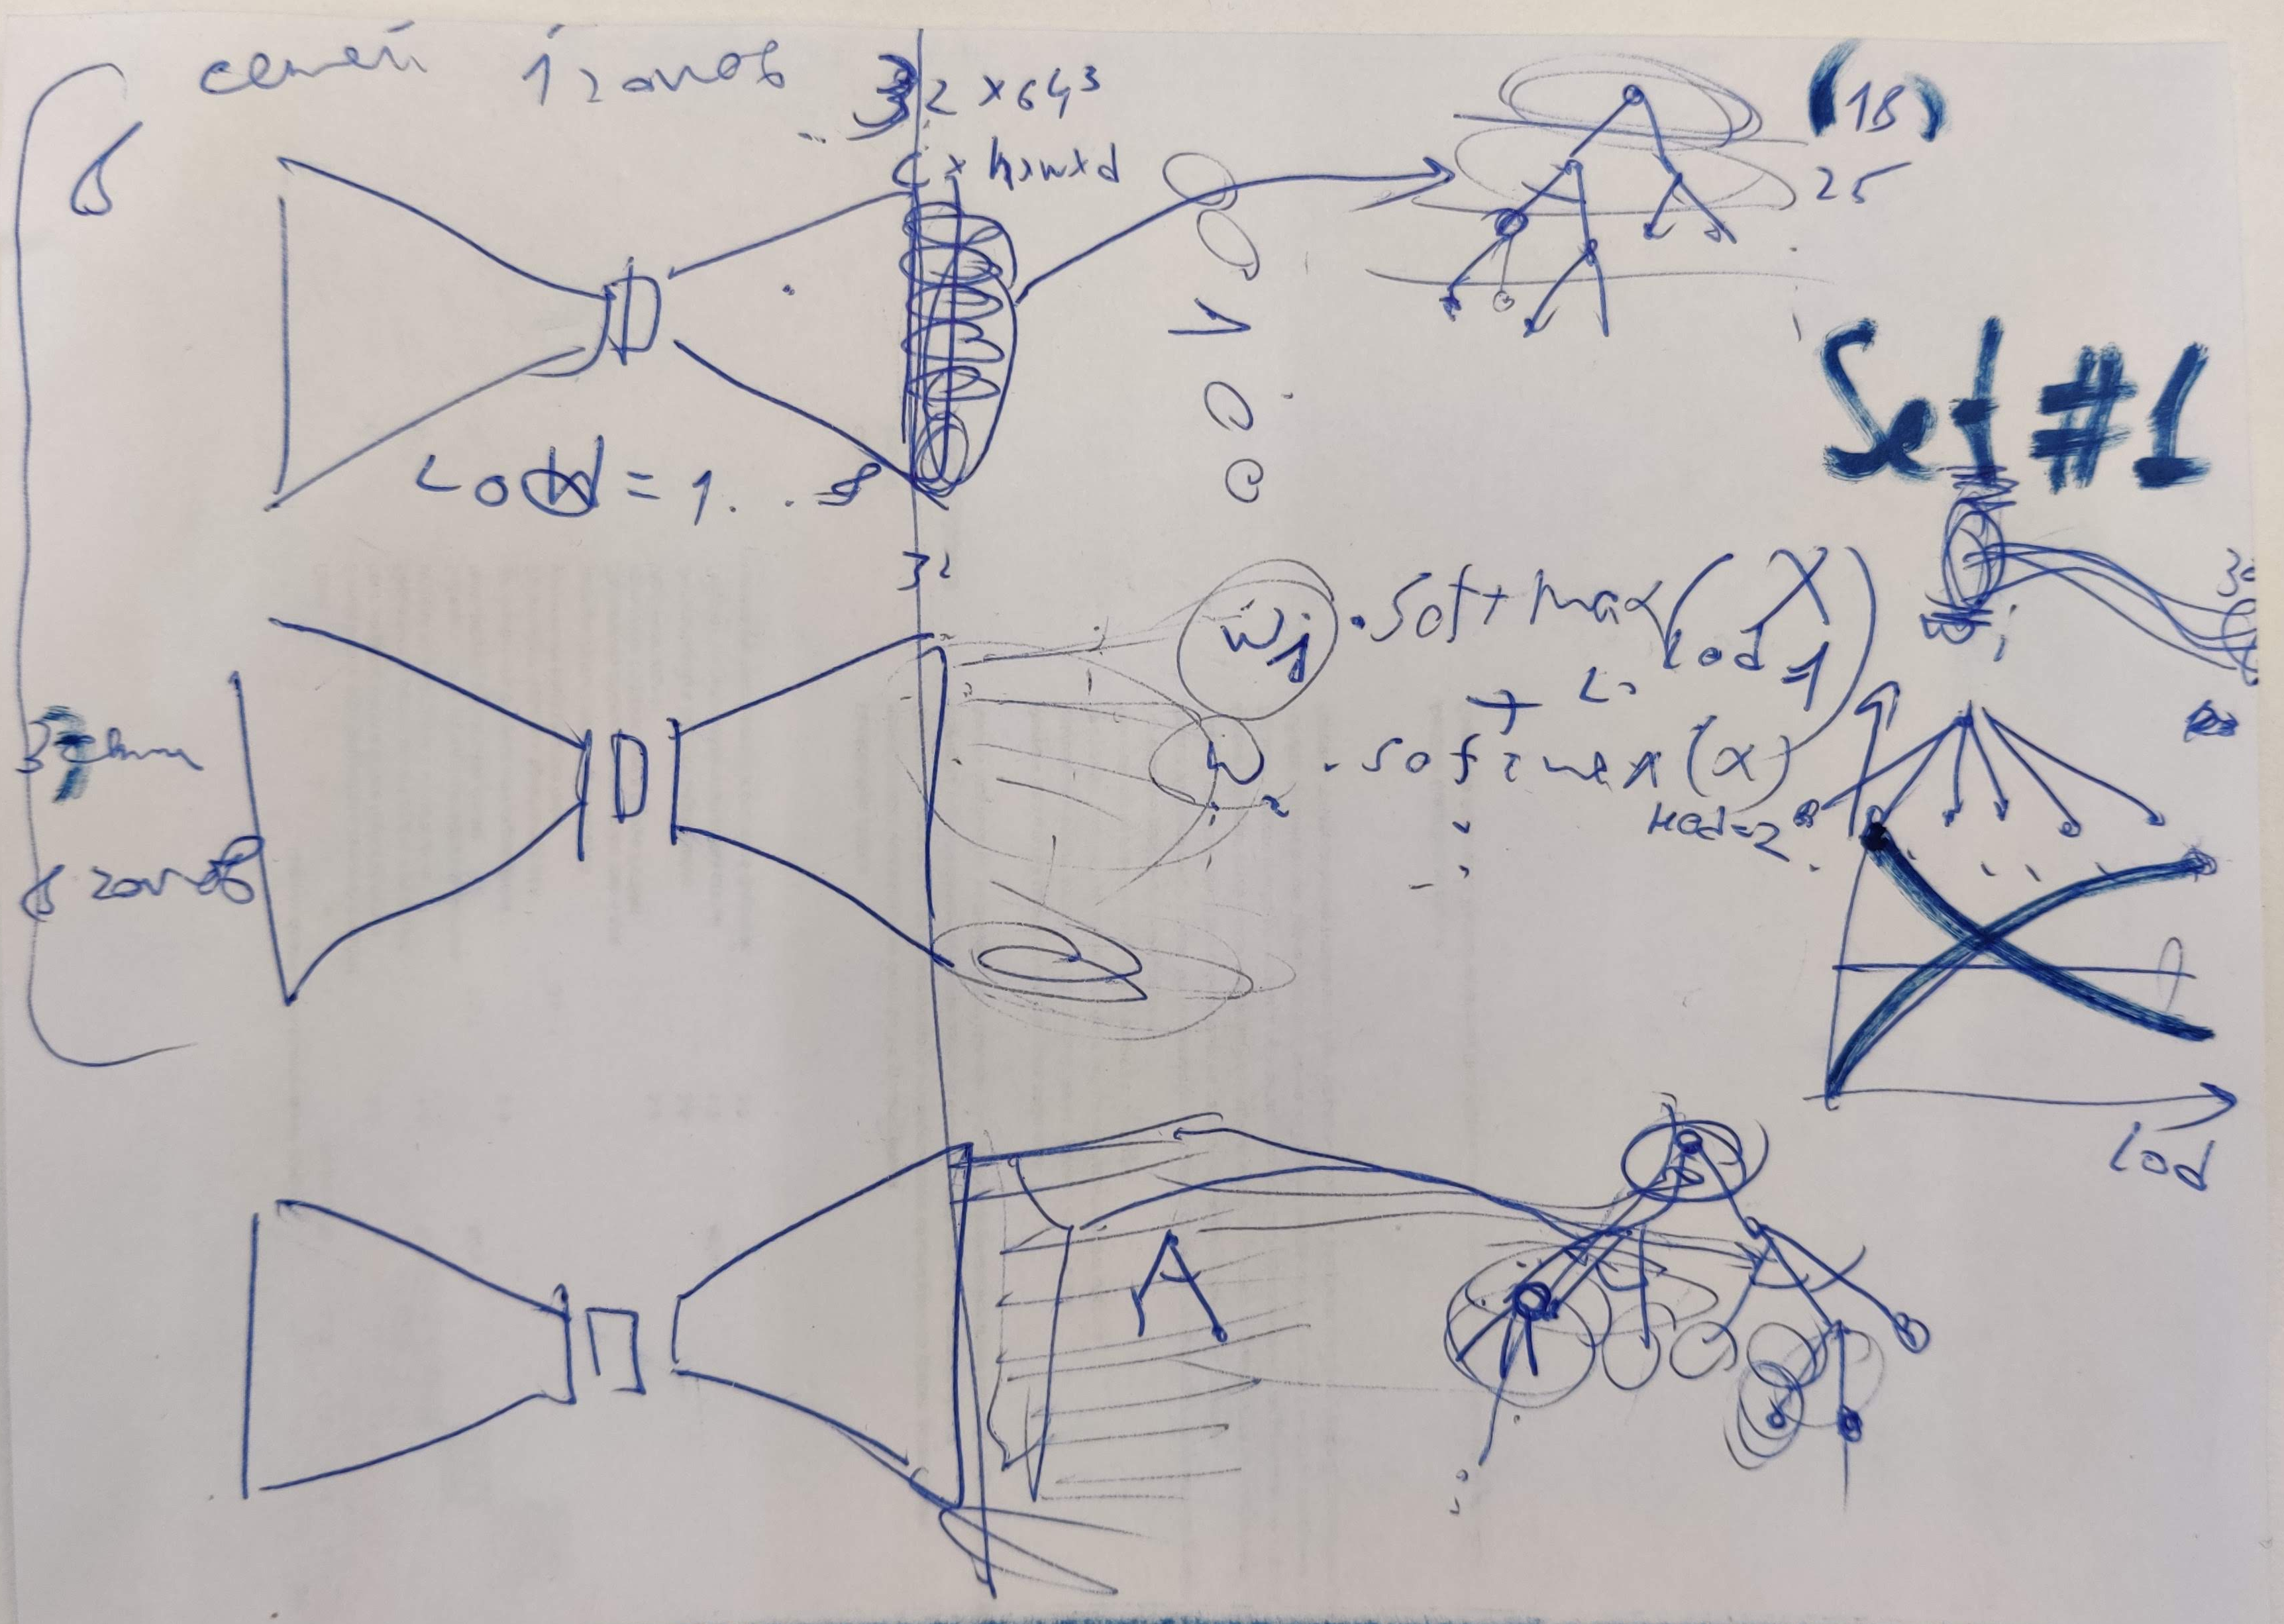
\includegraphics[trim=0 0 0 0, max width=\textwidth]{Figures/scan2part/architectures.pdf}
% \caption{Architectures of different segmentation models in different setups.}
% \end{figure}

% We compute a stratified train/test split, keeping split class ratios close to those in the whole dataset.
% Train and test sets were selected using combinatorial optimization routine that tries to split voxels of a class in ratios close to that of whole split.
We select 80\% of the scenes in ScanNet for training, keeping $1/16$ as a mini-validation to tune hyperparameters, and put aside 20\% scenes for testing.
During training, we extract 16~volumetric crops of size~$64^3$ from each voxelized scene and randomly shuffle them across all scenes in the training split.
% 16 crops were extracted from each scene, and shuffled with all other crops from other scenes.
The batch size we use ranges from 4 to 48 in different experiments, subject to fitting the network into the available GPU memory.
We optimize our models using Adam~\cite{kingma2014adam}, initalizing learning rate proportionally to the batch size, and decreasing it on pre-selected milestones by a factor $0.2$, with a weight decay of $10^{-4}$.
% for example for batch size = 32 base_lr=0.003, for bs=8 base_lr=0.001, for 48 base_lr=0.005 or 0.01 of it was too slow in training
We train until early stopping with patience parameter of 10, or until we reach a maximum epoch limit of 200.


% \DZ{unclear why different numbers where used}
% The encoder and the decoder consisted of 4 residual blocks each,  with output layers with  32 features for each voxel.
% Residual blocks included convolution, followed by ReLU non-linearity and group normalization with number of groups equal to 8.
% DZ already said this 
%Input tensors had only one channel the value of SDF function in that voxel.

\paragraph{Model configurations for different tasks}
\label{results:model_configs}
Table~\ref{table:configurations} summarizes our model specifications, differing by the choice of weights in~\eqref{eq:semseg_loss}.
To simplify the training process we assume all of the weights for loss functions to be normalized: $\sum_i \alpha_i = 1$.
